\subsubsection{Comparacion y Analisis de Modelos de Regresión}

La regresión es una técnica estadística que permite modelar y analizar las relaciones entre una variable dependiente y una o más variables independientes.

\begin{itemize}
    \item LinearRegression
    \item DecisionTreeRegressor
    \item KNeighborsRegressor
\end{itemize}

Para estos modelos, se utilizará la variable objetivo \say{sol1}, la técnica \say{K-Fold Cross-Validation}, ajustaremos el mejor modelo en los datos de entrenamiento y realizaremos predicciones utilizando el mejor modelo.

La mejor configuración para los modelos de regresión se en el siguiente codigo: \ref{lst:config_regresion}:

\begin{lstlisting}[language=Python, caption=Configuración de los modelos de regresión, label=lst:config_regresion]
# Definir los modelos de regresión
models_regresion = [
    LinearRegression(positive=True, fit_intercept=True),
    DecisionTreeRegressor(
        min_samples_split=5,
        min_samples_leaf=3,
    ),
    KNeighborsRegressor(n_neighbors=8),
]
    \end{lstlisting}

% -----------

\subsubsection{Selección de Características y Variable Objetivo}
Antes de entrenar los modelos, es crucial seleccionar las características que se utilizarán para la predicción y definir la variable objetivo. Esta selección garantiza que los modelos se entrenen con la información más relevante.

\begin{lstlisting}[language=Python, caption=Seleccion de caracteristica y variable objetivo, label=lst:config_varObjetivoCaracteristicas]
# Selección de características y variable objetivo para los modelos de Regresion.
y = df["sol1"]
X = df[
['hito1', 'hito2', 'exitosos', 'fallidos','e0', 'e1', 'e2', 'e3', 'e4', 'e5', 'e6', 'e7', 'e8', 'e9', 'e10', 'e11', 'e12', 'e13', 'e14', 'e15', 'e16', 'e17', 'e18', 'e19', 'e20', 'e21', 'e22', 'e23', 'e24', 'e25', 'e26', 'e27', 'e28', 'e29', 'e30', 'e31', 'e32', 'e33', 'e34', 'e35', 'e36', 'e37', 'e38', 'e39', 'e40', 'e41', 'e42', 'e43', 'e44', 'e45', 'e46', 'e47', 'e48', 'e49', 'e50', 'e51', 'e52']
]
\end{lstlisting}


% -----------
\subsubsection{Validación Cruzada y Entrenamiento}
La validación cruzada es una técnica que permite evaluar la capacidad de generalización de los modelos. En este estudio, se utiliza K-Fold Cross-Validation para entrenar y validar los modelos de regresión en diferentes subconjuntos del conjunto de datos.

\begin{lstlisting}[language=Python, caption=Configuraicones previas antes de la evaluación, label=lst:config_preEval]
# Listas para almacenar los resultados de cada modelo
mse_scores = []
mae_scores = []
r2_scores = []

best_model = None
best_mse = np.inf
best_mae = np.inf
best_r2 = -np.inf

# Colores para los modelos de regresión
colors = ["blue", "green", "red"]
    \end{lstlisting}

% -----------
\paragraph{Evaluación de Modelos de Regresión}
Una vez entrenados, es esencial evaluar el rendimiento de cada modelo. Esta evaluación se basa en métricas específicas que reflejan la precisión y eficacia de los modelos en la predicción de la variable objetivo.

\begin{lstlisting}[language=Python, caption=Codigo de evaluacion de modelos, label=lst:cod_Eval]
# Iterar sobre cada modelo de regresión
for i, model in enumerate(models_regresion):
    # Realizar k-fold cross-validation
    kf = KFold(n_splits=10, shuffle=True, random_state=1502)
    mse_cv_scores = []
    mae_cv_scores = []
    r2_cv_scores = []
    
    for train_index, test_index in kf.split(X):
        # Train-test split para cada fold
        X_train, X_test = X.iloc[train_index], X.iloc[test_index]
        y_train, y_test = y.iloc[train_index], y.iloc[test_index]
        
        # Entrenar el modelo
        model.fit(X_train, y_train)
        
        # Realizar predicciones en el conjunto de prueba
        y_pred = model.predict(X_test)
        
        # Calcular las métricas de evaluación
        mse = mean_squared_error(y_test, y_pred)
        mae = mean_absolute_error(y_test, y_pred)
        r2 = r2_score(y_test, y_pred)
        
        # Almacenar las métricas de evaluación para cada fold
        mse_cv_scores.append(mse)
        mae_cv_scores.append(mae)
        r2_cv_scores.append(r2)
        
    # Calcular la media de las métricas de evaluación para el modelo actual
    avg_mse = np.mean(mse_cv_scores)
    avg_mae = np.mean(mae_cv_scores)
    avg_r2 = np.mean(r2_cv_scores)
    
    # Almacenar las métricas de evaluación para el modelo actual
    mse_scores.append(avg_mse)
    mae_scores.append(avg_mae)
    r2_scores.append(avg_r2)
    
    # Verificar si el modelo actual es el mejor hasta ahora
    if avg_mse < best_mse:
        best_model = model
        best_mse = avg_mse
        best_mae = avg_mae
        best_r2 = avg_r2
    \end{lstlisting}

% -----------

\subsubsection{Resultados y Comparación}
Tras la evaluación, se presentan los resultados obtenidos de cada modelo. Estos resultados permiten identificar qué modelo tiene el mejor rendimiento en términos de precisión y eficacia.

Los resultados obtenidos se presentan en la Figura \ref{fig:metricas_regresion}:

\begin{figure}[H]
    \centering
    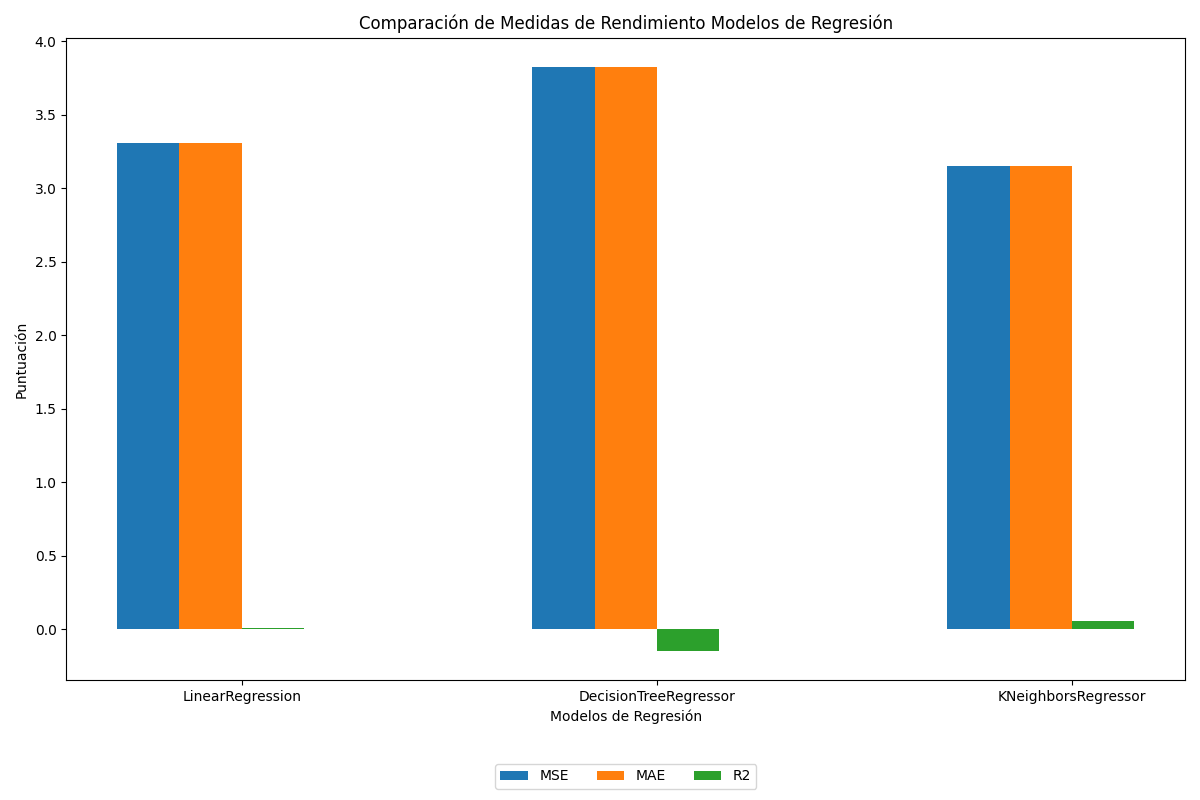
\includegraphics[width=1\textwidth]{img/compara_algoritmos/metricasEntreModelosRegresion.png}
    \caption{Métricas entre modelos de regresión conjunto de entrenamiento}
    \label{fig:metricas_regresion}
\end{figure}

Se observa que el modelo LinearRegression en su conjunto de entrenamiento presenta el comportamiento mas normal utilizando la validacion k-fold cross-validation para variables cuantitativas.
Para una visión más detallada y estructurada de estos resultados, se presenta la siguiente tabla:

\begin{table}[H]
    \centering
    \caption{Comparación de Métricas de Rendimiento para Modelos de Regresión}
    \begin{tabular}{lccc}
        \toprule
        \textbf{Modelo} & \textbf{MSE} & \textbf{MAE} & \textbf{R2 } \\
        \midrule
        Linear Regression & 0.6409 & 0.6300 & 0.5194 \\
        Decision Tree  & 0.6617 & 0.6446 & 0.5792 \\
        K-Neighbors & 0.6826 & 0.6761 & 0.5890 \\
        \bottomrule
    \end{tabular}
    \label{tab:res_metrics}
\end{table}

Los resultados sobre el conjunto de prueba se presentan en la figura \ref{fig:metricas_regresion_bestModel}

\begin{figure}[H]
    \centering
    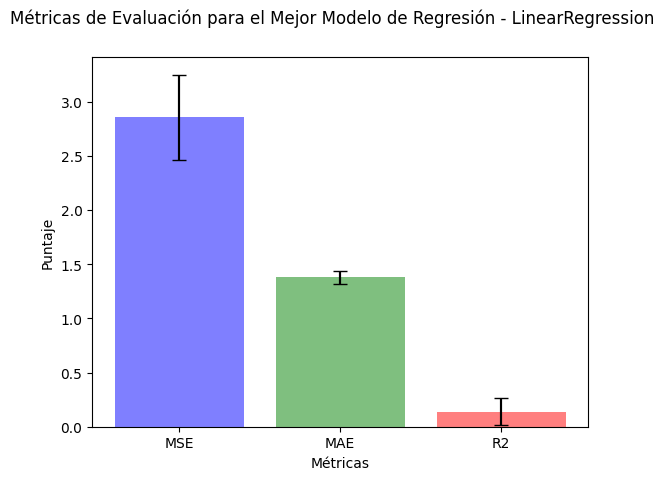
\includegraphics[width=0.7\textwidth]{img/compara_algoritmos/metricasBestModelLinearRegression.png}
    \caption{Métricas Best Model}
    \label{fig:metricas_regresion_bestModel}
\end{figure}

Se observa que el modelo LinearRegression es el mejor modelo de regresión, con un MSE del 3.6\% y un MAE del 1.6\%, valores inferiores a los de los otros modelos evaluados. Además, el modelo LinearRegression presenta un R2 más cercano a 1, con un aumento del 0.1\% en comparación con los demás modelos.

En base en los resultados obtenidos, se puede concluir que el modelo LinearRegression es el más adecuado para problemas de regresion con variable cuantitativas.

\begin{itemize}
    \item El mejor modelo en la validación fue: LinearRegression 14.1\%
\end{itemize}

Resultados del mejor modelo en el conjunto de prueba:

\begin{itemize}
    \item MSE: 3.6.\%
    \item MAE: 1.6\%
    \item R2: 0.1\%
\end{itemize}